% Compile with: pdflatex (run TWICE to resolve cross-references), or paste into Overleaf.
\documentclass[11pt]{article}
\usepackage[letterpaper, margin=1in, top=0.9in, bottom=0.9in]{geometry}
\usepackage[T1]{fontenc}
\usepackage[utf8]{inputenc}
\usepackage{mathpazo}
\usepackage{microtype}
\usepackage{hyphenat}
\usepackage{amsmath}
\usepackage{amssymb}
\usepackage{titlesec}
\usepackage{enumitem}
\usepackage{booktabs}
\usepackage{graphicx}
\usepackage{caption}
\usepackage{float}
\usepackage[authoryear,round]{natbib}
\usepackage{setspace}
\usepackage{hyperref}
\usepackage{xurl}
\hypersetup{colorlinks=true, linkcolor=black, citecolor=blue, urlcolor=blue}

\titleformat{\section}{\normalfont\large\bfseries}{\thesection.}{0.6em}{}
\titleformat{\subsection}{\normalfont\normalsize\bfseries}{\thesubsection.}{0.5em}{}
\titlespacing*{\section}{0pt}{0.6em}{0.2em}
\titlespacing*{\subsection}{0pt}{0.5em}{0.15em}

\captionsetup{font=small, labelfont=bf, skip=4pt}

\newcommand{\avgp}{\texttt{avg\_players}}

\setlength{\parskip}{0pt}
\setlength{\parindent}{2.5em}
\setlength{\emergencystretch}{3em}
\setlist{itemsep=0.2em, topsep=0.3em, partopsep=0pt, leftmargin=1.5em}

\begin{document}
\doublespacing

\begin{singlespace}
% ─────────────────────────── TITLE PAGE ────────────────────────────────────
\begin{center}
  {\LARGE\bfseries Epic Games Store Giveaways:\\[0.3em]
   Causal Effect on Steam Player Engagement}\\[1em]
  {\large Nicholas Liu}\\[0.4em]
  {\normalsize 14.33 | Spring 2026}\\[0.4em]
  % {\small MIT Department of Economics}
\end{center}

\vspace{0.8em}
\hrule
\vspace{1em}

% ─────────────────────────── ABSTRACT ──────────────────────────────────────
\begin{center}
  \textbf{Abstract}
\end{center}

\noindent Does a free game giveaway on the Epic Games Store increase or decrease
engagement for the same title on Steam? Using a staggered
difference-in-differences event study across 446 treated games from
2018--2025, we estimate a two-phase dynamic. In the giveaway month, Steam
concurrent players rise by approximately 10--14\% across TWFE, LP-DiD, and
stacked DiD; the effect then reverses, with twelve-month point estimates
spanning roughly $0$ to $-27\%$ depending on estimator. The preferred
stacked-DiD specification attenuates to near zero by the end of the window.
A pre-trend test rejects parallel trends in low-traffic titles, suggesting
lifecycle-decline selection inflates the medium-run negatives. We read the
short-run spike as evidence of an advertising mechanism, and the medium-run
estimates as an upper bound on any causal substitution effect.

\vspace{0.5em}
\noindent\textit{Keywords:} platform competition, cross-platform spillovers, video games, Epic Games Store, Steam

\vspace{1em}
\hrule
\vspace{1em}
\end{singlespace}

% ─────────────────────────── 1. INTRODUCTION ───────────────────────────────
\section{Introduction}

When most gamers hear about a new video game, their first instinct is to open Steam
and search for it. This reflects the social ecosystem Steam has cultivated: friend
lists, community hubs, reviews, achievements, and wishlist notifications so
comprehensive that it functions not only as a store but as the primary discovery and
identity layer for PC gaming. Even a game distributed \textit{entirely for free} on a
rival platform is liable to drive curious players to Steam first.

This intuition recently received vivid anecdotal support. In January 2026, the CEO of
New Blood Interactive shared that when \textit{Blood West} was given away for free on
the Epic Games Store over the 2025 holiday period, Steam sales for the title surged
by approximately 200\% on the same day \citep{frvr2026}. ``I used to think EGS was a
Marketing Black Hole,'' he wrote, ``but turns out having your game be free on Epic is
great advertising for Steam sales!'' The comment went viral, sparking a Reddit thread
that generated broad discussion of whether the Epic giveaway program systematically
benefits Steam rather than draining it \citep{reddit2026}.

These observations raise a causal question: does an Epic Games Store free giveaway
increase or decrease engagement for the same game on Steam? Standard substitution
logic predicts a decrease: a zero-price substitute on a rival platform should divert
players away from Steam. Yet the anecdotal evidence points in the opposite direction
in the short run. The giveaway may function as an advertising shock: it generates
media coverage, social-media chatter, and word-of-mouth that raise awareness of the
title and drive traffic to Steam, the platform where players already hold a
library, social graph, and community history.

The PC gaming platform market is a compelling context. Steam, launched by Valve in
2003, remains overwhelmingly dominant with more than 120 million monthly active users
and a catalogue exceeding 50{,}000 titles as of 2025; its competitive moat rests not
only on library size but on the thick social infrastructure that creates switching
costs no price cut can replicate. The Epic Games Store, launched in December 2018 on
the back of \textit{Fortnite}'s revenue, has pursued an aggressive free-game strategy
as its primary differentiation lever, giving away more than 400 games at no cost to
users since launch.

Against this backdrop, this paper estimates the causal effect of EGS giveaways on
Steam player engagement using a staggered difference-in-differences event study
across 446 games given away between December 2018 and 2025. The identifying variation
is the timing of each game's first EGS giveaway: games awaiting future giveaways
serve as not-yet-treated controls for currently treated games, exploiting the rolling
staggered rollout of the Epic program rather than relying on an external never-treated
comparison. Engagement is measured via monthly average concurrent players scraped from
SteamCharts.

The central empirical finding is a two-phase dynamic. In the giveaway month and the
month after, Steam player counts rise by approximately 10--14\% in log terms; the
contemporaneous spike is statistically significant ($p<0.001$) across all three
estimators (TWFE, LP-DiD, and stacked DiD) and passes a randomization placebo. The
effect then reverses within a few months, but how far is estimator-dependent: TWFE
and LP-DiD reach roughly $-11\%$ to $-27\%$ by month twelve, while the preferred
stacked-DiD specification flattens to a statistically insignificant $+0.016$. The spread brackets the medium-run causal
substitution effect between essentially zero and $-27\%$, with the true magnitude
likely closer to the lower end because all three estimators absorb pre-existing
lifecycle decline only imperfectly. Repeat giveaways of the same game generate no
detectable additional effect.

We interpret this as advertising plus selection. The $k = 0$ spike is consistent
with the giveaway announcement attracting attention to the title on Steam. The
medium-run negatives are partly contaminated by selection: the full-sample
pre-period joint Wald test does not reject parallel trends at the 5\% level
($F_{11,444}=1.72$, $p=0.067$), but the point estimates drift downward toward
$k=-1$, and the low-traffic subsample does reject ($F_{11,213}=1.89$, $p=0.042$).
Any genuine causal substitution component is therefore best read as an upper bound.
The central contribution is the large-scale causal estimate of the full dynamic
trajectory of cross-platform spillovers from free-game promotions (446 games,
38{,}641 game-month observations, seven years of history), including the sustained
post-giveaway reversal that prior work has not characterized.

% ─────────────────────────── 2. LITERATURE REVIEW ──────────────────────────
\section{Literature Review}
\label{sec:lit}

The most directly related work is \citet{clarkson2025}, a doctoral dissertation
whose second chapter finds that games given away by Epic see Steam traffic
increase by more than 24\% during the giveaway window, with concurrent rises in
Steam reviews and word-of-mouth activity, and larger spillovers for titles that
lean on Steam-exclusive features. The present paper differs in three respects:
it estimates the full twelve-month post-treatment trajectory using a staggered DiD
design across 446 games and seven years of history (rather than only the
contemporaneous effect on a curated sample), uses three heterogeneous-treatment-robust
estimators to bracket the causal effect, and documents both the systematic medium-run
reversal and the pre-period drift that points to lifecycle-decline selection, a
mechanism invisible to a contemporaneous design. 

More broadly, the question fits
into the literature on platform competition and multi-homing in two-sided markets
\citep{rochet2003}: when two platforms primarily serve the same user base, a free
promotion on one may simply reallocate engagement rather than expand the aggregate
market. \citet{tudon2022} estimates a 0.13\% own-demand response per 1\% rise in
friends' Steam demand, providing a network-multiplier channel through which a free
copy on a rival platform can lift incumbent-platform engagement; \citet{nabil2025}
document that Steam's content-variety and ease-of-use advantages over EGS persist
despite Epic's free-game program, consistent with a durable Steam incumbency
advantage rooted in its community infrastructure rather than price.

% ─────────────────────────── 3. DATA ───────────────────────────────────────
\section{Data}
\label{sec:data}

\subsection{Epic Giveaway History}

We obtained a Kaggle dataset \citep{dongre2025} recording every free game offered through
the Epic Games Store from December 2018 through 2025, comprising 541 giveaway events
corresponding to 471 unique game titles; the remaining 70 events are repeat
appearances.\footnote{The source dataset flags repeat appearances with a
``(repeat)'' suffix appended to the game name. Nine titles had this suffix
incorrectly applied to their first appearance; we manually corrected these so that
only genuine repeats carry the suffix.} Repeats cluster in two patterns:
\textit{distant repeats}, where a game is offered again more than twelve months
after its first appearance, and \textit{proximate repeats}, where the same game
is offered within a few months or even days of the first, most notably during
Epic's annual holiday giveaway batches.\footnote{The longest gap is 57 months
(\textit{Kingdom Come: Deliverance}); the shortest are gaps of a few days
inside the same holiday batch.} Table~\ref{tab:epic_csv} summarizes the
giveaway structure; we retain all giveaway dates for each game to support the
multi-event analysis.

\subsection{SteamCharts Monthly Player Data}

For each Epic giveaway title matched to a Steam App ID, we scraped monthly
average and peak concurrent player counts from
\texttt{steamcharts.com/app/\{appid\}}.\footnote{SteamCharts renders its
historical tables server-side, so standard HTTP requests suffice.} The overall
panel spans July 2012 through February 2026, but each game's time series begins
only from the month it first appeared on SteamCharts (typically near its Steam
release date). The median game has 88 months of data.

\subsection{Merge Pipeline}

Matching Epic game names to Steam App IDs required reconciling inconsistent
titling such as subtitles, punctuation, and edition suffixes; Table~\ref{tab:pipeline}
summarizes the pipeline.\footnote{RapidFuzz fuzzy string matching auto-matched
413 of 471 unique names; the remaining 58 received manual review (50 resolved,
8 confirmed absent from Steam). Fifteen matched entries are DLC or in-game
content mapped to the base-game App ID.}

\subsection{Final Panel and Summary Statistics}

The assembled dataset contains 38{,}642 game-month observations across 446
games.\footnote{One observation is dropped by the TWFE estimator as a singleton
fixed effect, leaving an effective regression sample of 38{,}641 game-months.}
The outcome variable is $\ln(\avgp+1)$, where \avgp{}
is the SteamCharts monthly average concurrent player count; the $+1$ offset
accommodates zero-player months and the log transformation compresses the heavy
right tail driven by a small number of AAA titles.

Table~\ref{tab:sumstats} reports summary statistics: the raw player count is
highly right-skewed (mean $1{,}584$, median $65$), reflecting a long-tail indie
distribution with occasional blockbusters, and the log-transformed outcome is
far better behaved (mean 4.43, SD 2.36). Figure~\ref{fig:outcome} compares the
pre- and post-giveaway distributions of the outcome and its unconditional mean
by event-time, with a sharp uptick visible at $k = 0$; Figure~\ref{fig:desc}
characterises the panel's structure (pre-treatment log-player distribution,
the broadly even spread of treatment cohorts across 2019--2023, and the
fraction of each cohort flagged as repeat).\footnote{17 games have no
pre-period observations and are omitted from Panel (a) of Figure~\ref{fig:desc};
the repeat-indicator series in Panel (c) is based on any repeat, proximate or
distant, so it exceeds the 30-game proximate-repeat count in
Table~\ref{tab:epic_csv}.}

% ─────────────────────────── 4. EMPIRICAL METHOD ───────────────────────────
\section{Empirical Method}
\label{sec:method}

\subsection{Identification Strategy}

The identifying variation is the timing of each game's first Epic giveaway
across 80 distinct calendar months spanning December 2018 through late
2025.\footnote{For the stacked DiD and Callaway--Sant'Anna estimators these
treatment months are aggregated into 29 quarterly cohorts.} Because the Epic program has cycled continuously through a broad
catalogue of genres and release-years, games awaiting future giveaways serve as
natural controls for currently treated games.\footnote{An external never-treated
control group was not constructed because doing so would require scraping
SteamCharts data for a large subset of the $\sim$50{,}000 non-EGS Steam titles
without a principled sampling frame; any criterion for choosing which to include
risks biasing the comparison toward stable-trajectory titles.}

The key identifying assumption is parallel trends: in the absence of treatment,
the log player trajectory of games in different giveaway cohorts would have
followed the same path after conditioning on game and calendar-month fixed
effects.

\subsection{Pooled TWFE Specification}

The primary specification is a two-way fixed-effects (TWFE) event-study regression on
the full unbalanced game-month panel:
\begin{equation}
\label{eq:pooled}
\ln(y_{it} + 1) = \alpha_i + \gamma_t +
  \sum_{\substack{k \in [-12,\,12] \\ k \neq -1}}
  \theta_k \cdot \mathbf{1}[\tilde{k}_{it} = k]
  + \varepsilon_{it}
\end{equation}
where $\alpha_i$ are game fixed effects, $\gamma_t$ are calendar-month fixed
effects, $\tilde{k}_{it} = \text{clip}(k_{it},\,-12,\,12)$ is event-time
clipped to the $[-12, 12]$ window, and the omitted category is $k = -1$.
$\hat{\theta}_k$ estimates the average change in log Steam players at
event-time $k$ relative to the pre-giveaway baseline, pooling first and repeat
events per game. Standard errors are clustered at the game level. Staggered
treatment across 80 distinct treatment months identifies $\theta_k$ separately
from $\gamma_t$, so the omitted reference $k = -1$ suffices despite the absence
of a never-treated group. Rather than restrict to the 336 full-window games, we
retain all 446 by clipping event-time: $k < -12$ enters the $k = -12$ bin and
$k > 12$ enters the $k = 12$ bin, so the boundary-bin estimates at $\pm 12$
should be read as averages over all periods beyond the window. Re-estimating
Equation~\eqref{eq:pooled} on the 336-game full-window subsample yields
qualitatively identical results.

\subsection{Robustness Estimators}

Because treatment timing is staggered across six years, the standard TWFE estimator
is potentially biased when treatment effects are heterogeneous across cohorts
\citep{callaway2021}. We complement it with two heterogeneous-treatment-robust
event-study estimators reported alongside TWFE in Section~\ref{sec:results}, plus
a Callaway--Sant'Anna cohort-ATT analysis whose construction sacrifices precision
for the strongest negative-weighting protection and is therefore deferred to
Appendix~\ref{app:csatt}, with the per-cohort decomposition in
Appendix~\ref{app:cohort_paths}.

\textbf{LP-DiD \citep{dube2023}.} For each event time $k$, LP-DiD runs a separate
local-projection regression of the change in log players from $k = -1$ to $k$ on
treatment, restricting controls to games not yet treated as of calendar time
$t + k$. This avoids the negative weights TWFE assigns to already-treated
comparators under heterogeneous effects.\footnote{The requirement that controls
remain untreated through the outcome period means that at large $k$ the eligible
control pool shrinks to games whose giveaway is still many months away. All
cohorts are pooled within each $k$-specific regression, with cohort fixed
effects absorbing calendar-time differences across cohorts; standard errors are
clustered by game.}

\textbf{Stacked DiD \citep{cengiz2019}.} For each treatment
cohort $g$ (quarter of first giveaway) we form a balanced panel of cohort-$g$
games with event-time $k \in [-12, 12]$ alongside not-yet-treated games observed
over the same calendar window, and estimate
\begin{equation}
\label{eq:stacked}
\ln(y_{ist} + 1)
= \alpha_{is}
+ \mu_{sc_t}
+ \sum_{k \neq -1} \beta_k \cdot \mathbf{1}[\tilde k_{ist} = k] \cdot \text{treated}_{is}
+ \varepsilon_{ist},
\end{equation}
where $s$ indexes the stack, $\alpha_{is}$ is a unit-within-stack fixed effect,
and $\mu_{sc_t}$ is a stack-by-calendar-month fixed effect that absorbs aggregate
shocks within each cohort.\footnote{Interacting the event-time dummies with the
treated indicator ensures $\beta_k$ is identified only from the differential
trajectory of treated units relative to not-yet-treated controls inside each
$(s, c_t)$ cell. Games appearing in multiple stacks are weighted by
$1/n_{\text{stacks}}$; standard errors are clustered by game.} Stacked DiD with
stack-by-calendar-month FE is our preferred causal estimator because it most
fully neutralizes both control-composition bias and aggregate calendar-time
shocks; LP-DiD and TWFE are reported alongside it as bracketing estimates
likely inflated by any pre-existing lifecycle decline.

% ─────────────────────────── 5. RESULTS ────────────────────────────────────
\section{Results}
\label{sec:results}

\subsection{TWFE Event Study}
\label{ssec:twfe}

Figure~\ref{fig:compare} presents the pooled TWFE event-study
coefficients $\hat{\theta}_k$ from Equation~\eqref{eq:pooled}, with 95\%
confidence intervals clustered at the game level. Table~\ref{tab:coefs} reports
selected coefficients; the full 24-coefficient table is in
Appendix~\ref{app:coeftable}. In the giveaway month ($k = 0$), $\hat{\theta}_0 = 0.101$
(SE = 0.022, $p < 0.001$), implying approximately a 10.6\% increase in Steam
concurrent players. The effect remains marginally positive at $k = 1$
($\hat{\theta}_1 = 0.045$, $p = 0.047$) but turns negative and highly significant
from $k = 2$ onward, reaching $-0.145$ (13.5\% below baseline) by $k = 5$ and
$-0.267$ (23.4\% below baseline) by $k = 12$. The pre-period coefficients
($k \in [-12, -2]$) are not individually statistically distinguishable from
zero but visually appear to drift downward toward $k = -1$.

\subsection{Estimator Comparison}
\label{ssec:compare}

Figure~\ref{fig:compare} overlays the TWFE, LP-DiD, and stacked-DiD event-study
paths and Table~\ref{tab:estimator_compare} reports key coefficients.
Qualitatively all three estimators show the same two-phase pattern: a positive
spike at $k = 0$ that persists into $k = 1$, a reversal at $k = 2$, and
statistically significant negatives by $k = 5$. The pre-period coefficients drift
downward across the window but are not individually statistically distinguishable
from zero given the standard errors.

The estimators diverge sharply on the medium-run magnitude. At $k = 12$, TWFE
reaches $-0.267$, LP-DiD $-0.105$, and stacked DiD a statistically insignificant
$+0.016$. The contemporaneous estimates are tighter (TWFE and stacked both
$+0.101$, LP-DiD $+0.131$); LP-DiD's slightly larger $k = 0$ estimate reflects
that its not-yet-treated controls are EGS-selected games approaching their own
giveaway and so are themselves in the steepest phase of pre-treatment lifecycle
decline, mechanically inflating the DiD contrast. The systematic pattern across
the medium-run window is that the more aggressively an estimator absorbs
calendar-time shocks within cohort stacks (stacked DiD $>$ LP-DiD $>$ TWFE in
that dimension), the smaller the medium-run negative becomes. The
three-estimator spread therefore brackets the medium-run causal substitution
effect between roughly $0$ and $-27\%$, with the preferred stacked-DiD point
estimate at the less-negative end and losing statistical significance by
$k = 12$. We return to interpretation in Section~\ref{sec:discussion}.

\textbf{Pre-trend test.}\label{ssec:pretrend}
The joint pre-trend Wald test evaluates $H_0: \theta_k = 0$ for all
$k \in [-12, -2]$ using the full clustered covariance matrix of the TWFE
coefficient vector. On the full sample the joint Wald statistic is
$\chi^2_{11} = 18.89$ with $p = 0.063$, or equivalently $F_{11, 444} = 1.72$
with $p = 0.067$, failing to reject zero pre-trends at the conventional $5\%$
level but rejecting at $10\%$. The high-traffic subsample is a clean failure
to reject ($\chi^2_{11} = 9.04$, $p = 0.618$; $F_{11, 214} = 0.82$),
consistent with stable pre-trends in larger titles. The low-traffic subsample,
by contrast, rejects parallel trends at $5\%$: $\chi^2_{11} = 20.82$,
$p = 0.035$ ($F_{11, 213} = 1.89$, $p = 0.042$). The pre-trend violation is
therefore concentrated in lower-traffic titles, where lifecycle decline is
more pronounced; we return to the implications in
Section~\ref{sec:discussion}.

\textbf{Separated specification.} A separated specification distinguishing
first-giveaway from repeat-giveaway effects yields a null repeat coefficient
and leaves the first-event path numerically identical to the pooled
$\hat{\theta}_k$; full specification, results, and interpretation are in
Appendix~\ref{app:separated}.

\subsection{Popularity-Stratified Analysis}
\label{ssec:pop}

We split the sample at the pre-treatment median of average Steam players (59.2
players/month) into 215 high-traffic and 214 low-traffic games and estimate
Equation~\eqref{eq:pooled} separately for each half.\footnote{The 17 games
with no pre-period observations in our panel have no defined pre-treatment
median and contribute only to the pooled specification.}
Figure~\ref{fig:popularity} presents the event-study estimates. High-traffic
games exhibit a cleaner pattern: a larger and more precisely estimated spike
at $k = 0$ and a statistically clean pre-period, while low-traffic games are
noisier and reject parallel trends, as documented by the pre-trend Wald
statistics in Section~\ref{ssec:pretrend}. The selection-on-decline concern
is therefore more concentrated in this stratum. Otherwise, the qualitative
two-phase dynamic is present in both strata.

\subsection{Robustness Checks}

Three additional checks confirm the main pattern. The clean-sample
re-estimation drops the 30 games with a proximate repeat giveaway; the
holiday-batch re-estimation drops the 73 games whose first giveaway falls in
one of Epic's December ``15 days of free games'' batches; and a randomization
placebo permutes treatment dates 200 times to construct an empirical null for
the contemporaneous spike. All three leave the headline TWFE path essentially
unchanged. Full results are in Appendices~\ref{app:robustness},
\ref{app:holiday}, and~\ref{app:placebo}.

% ─────────────────────────── 6. DISCUSSION ─────────────────────────────────
\section{Discussion}
\label{sec:discussion}

\subsection{Interpreting the Contemporaneous Spike}

The $k = 0$ and $k = 1$ positive effects are consistent with the Epic giveaway
functioning as an advertising shock that temporarily lifts Steam engagement.
A free-game announcement generates media coverage and social-media chatter, and
because Steam is the primary discovery and community layer for PC games, the
resulting awareness surge manifests as Steam activity even when players also
claim the free Epic copy. The magnitude (roughly 10--14\% in log players) is in
the same direction as but smaller than the $\approx 24\%$ found by
\citet{clarkson2025}, who measures Steam traffic in the days immediately
after the giveaway window on a sample weighted toward larger titles, whereas
we measure monthly average concurrent players and include near-zero-engagement
games.

\subsection{Interpreting the Reversal}

The sustained reversal from $k = 2$ through $k = 12$ is the most novel
finding, and two mechanisms likely contribute. First, Epic's curation team
may preferentially select titles whose Steam player base is already
declining,\footnote{Plausibly because declining games are cheaper to license,
or because publishers of fading titles are more willing to accept giveaway
terms.} so part of the observed post-giveaway decline may continue a
pre-existing downward trend rather than reflect a causal consequence. The
evidence is suggestive: the pre-trend tests in Section~\ref{ssec:pretrend}
localize the concern to low-traffic titles, and the stacked estimator
produces a much smaller medium-run negative than TWFE, consistent with part
of the TWFE path being a selection artefact. Selection cannot, however,
explain the contemporaneous spike at $k = 0$, which is robustly causal across
estimators and passes the randomization placebo.

Second, players who claimed the free Epic copy may gradually shift playtime
from Steam to Epic, or may forgo a Steam purchase they would otherwise have
made, leaving Steam with a permanently lower post-treatment
baseline.\footnote{The substitution channel predicts a reversal beginning at
$k \geq 2$ rather than $k = 0$ because players need time to install and play
the game they claimed.} The ordering of medium-run estimates across
estimators (TWFE most negative, stacked DiD smallest) is consistent with both
mechanisms operating jointly: if selection is the dominant non-causal driver,
the stacked-DiD path is the cleanest view of the causal substitution effect,
which is close to zero by $k = 12$, and TWFE and LP-DiD at $k = 12$ should be
read as upper bounds.

\subsection{Implications for Platform Strategy}

For developers, the calculus is reasonably clear once the components are
separated. Any pre-existing lifecycle decline would continue regardless of the
giveaway and should not enter the decision. The substitution component imposes
little real cost on the developer: a player who migrates from Steam to Epic is
still playing the game, and Epic's 12\% revenue cut is more favorable than
Steam's 30\%. The deal therefore reduces to two clearly positive terms, the
upfront licensing fee and the advertising spike (our estimated $+10$--$14\%$
at $k = 0$), and is typically favorable for a developer whose title is
declining or past peak.\footnote{\citet{clarkson2025} documents that Steam
reviews rise alongside players during giveaways, feeding the recommendation
algorithm, and the Blood West case \citep{frvr2026} suggests the
purchase-conversion effect can far exceed the engagement effect.}

For Steam, the program appears to be a net positive rather than a threat. The
$k = 0$ advertising spike accrues directly to Steam, and the medium-run
negatives are likely upper bounds (with the preferred stacked-DiD estimate near
zero by $k = 12$). The deeper observation is that even free distribution
through a rival platform funnels players to Steam's community layer, consistent
with the view that Steam's moat is rooted in library, friends, and community
activity rather than price.

For Epic, the picture is more ambiguous and our data can only partially answer
it. Epic bears the full licensing cost; the measurable engagement effects of
the giveaway accrue to Steam. What Epic plausibly gains instead is EGS user
acquisition: launcher installs, repeat visits, and eventual paid purchases,
none of which is observable in Steam-side data. If the primary measurable
effect of Epic's giveaway spending is to advertise games on a competitor's
platform, whether the program is strategically rational hinges on EGS
user-acquisition gains that this paper cannot test.

\subsection{Limitations}

The two most consequential limitations are intertwined. First, there is no
never-treated group: all 446 games are eventually treated, so identification
rests entirely on timing variation across cohorts (see Section~\ref{sec:method}
for why an external never-treated pool was not constructed). A well-constructed
never-treated comparison could in principle sharpen identification.
Second, Epic may preferentially select games already in lifecycle
decline, violating parallel trends for the post-giveaway reversal. The
pre-trend evidence reported in Section~\ref{ssec:pretrend} is consistent with
selection concentrated in low-traffic titles. The TWFE and LP-DiD medium-run estimates
should therefore be read as upper bounds on the true causal substitution
effect; the stacked-DiD estimate of $+0.016$ at $k = 12$ is the closest to a
causal estimate our design can produce but is statistically insignificant.
Three further limitations apply to measurement and external validity.
\textit{Player counts vs.\ purchases.} SteamCharts reports concurrent players,
not purchases or unique installs; a giveaway effect on purchases may be larger
than, or differently timed from, the player-count effect we estimate.
\textit{DLC and bundle giveaways.} Fifteen events distributed DLC or in-game
content rather than the base game; mapping these to the base game's App ID
likely attenuates the estimated effect for those observations.
\textit{Genre heterogeneity.} The Epic catalogue mixes single-player titles
(where the substitution mechanism is weaker) and multiplayer titles (where
platform choice has ongoing matchmaking consequences); the pooled estimate
conflates these. A genre-stratified analysis is deferred to future work, with
the popularity split in Section~\ref{ssec:pop} serving as a partial proxy.

% ─────────────────────────── 7. CONCLUSION ─────────────────────────────────
\section{Conclusion}
\label{sec:conclusion}

Using 446 games over 2018--2025 and a staggered difference-in-differences
design, this paper estimates the full trajectory of Steam player engagement
around Epic Games Store free giveaways. The pattern is two-phase: a
short-run advertising spike of approximately 10--14\% in log players at
$k = 0$--$1$ that is robust across estimators and a randomization placebo,
followed by a medium-run reversal whose magnitude depends on how aggressively
the estimator absorbs cohort-level shocks. The reversal is partly contaminated
by selection on lifecycle decline: the pre-trend violation localises to
low-traffic titles, and the preferred stacked-DiD estimate flattens to a
statistically insignificant $+0.016$ by $k = 12$. The medium-run causal
substitution effect is therefore plausibly small; Epic's giveaway program
appears to function in part as inadvertent Steam advertising.

Future work could separate single-player from multiplayer titles to test
whether substitution is stronger where platform choice is more permanent;
study Steam sales volume rather than concurrent players to quantify
commercial impact directly; and examine whether giveaways generate lasting
EGS engagement using Epic's own platform data, which is not publicly
available.

\clearpage

% ═══════════════════════════════════════════════════════════════════════════
%  TABLES & FIGURES
% ═══════════════════════════════════════════════════════════════════════════

\begin{singlespace}

\begin{center}
{\large\bfseries Tables \& Figures}
\end{center}

\vspace{1em}

\begin{table}[H]
\centering\small
\caption{Epic Games Store giveaway CSV breakdown (Dec 2018--2025)}
\label{tab:epic_csv}
\begin{tabular}{lc}
\toprule
Category & Count \\
\midrule
Total giveaway events & 541 \\
\quad First appearances (unique titles) & 471 \\
\quad Repeat appearances & 70 \\
\midrule
\multicolumn{2}{l}{\textit{Of 63 titles given away more than once:}} \\
\quad Given away exactly twice & 56 \\
\quad Given away three times & 7 \\
\midrule
\multicolumn{2}{l}{\textit{Of 63 repeat titles, by gap to first giveaway:}} \\
\quad Proximate ($\leq$12 months) & 30 \\
\quad Distant ($>$12 months) & 33 \\
\bottomrule
\end{tabular}
\end{table}

\vspace{2em}

\begin{table}[H]
\centering\small
\caption{Steam matching pipeline and final panel construction}
\label{tab:pipeline}
\begin{tabular}{lc}
\toprule
Stage & Count \\
\midrule
Unique Epic titles (input to matching) & 471 \\
\quad Matched to a Steam app ID & 463 \\
\quad Not on Steam: Epic exclusives & 5 \\
\quad Not on Steam: placeholder entries & 3 \\
\midrule
\multicolumn{2}{l}{\textit{Of 463 matched entries:}} \\
\quad Unique Steam app IDs & 459 \\
\quad Duplicate collisions (different Epic name, same app ID) & 4 \\
\midrule
No SteamCharts data (HTTP 500) & 13 \\
\textbf{Games in final panel} & \textbf{446} \\
\quad Treatment month observed in SteamCharts & 421 \\
\quad Full $[-12,+12]$ window observed in SteamCharts & 336 \\
\bottomrule
\end{tabular}
\end{table}

\vspace{2em}

\begin{table}[H]
\centering\small
\caption{Summary statistics: Epic giveaway panel}
\label{tab:sumstats}
\begin{tabular}{lrccccc}
\toprule
Variable & $N$ & Mean & SD & Min & Median & Max \\
\midrule
Avg.\ concurrent Steam players (monthly) & 38,642 & 1,583.9 & 7,444.0 & 0.00 & 65.2 & 270,553 \\
Peak concurrent Steam players (monthly)  & 38,642 & 3,214.1 & 14,861.2 & 0 & 171 & 527,652 \\
$\ln(\avgp+1)$ [outcome] & 38,642 & 4.43 & 2.36 & 0.00 & 4.19 & 12.51 \\
Repeat-giveaway window indicator (0/1)   & 38,642 & 0.02 & 0.15 & 0 & 0 & 1 \\
\midrule
Months of SteamCharts data per game & 446 & 86.6 & 41.1 & 1 & 88 & 163 \\
\bottomrule
\end{tabular}
\medskip

\noindent\small\textit{Notes:} Game--month panel, 446 games, July 2012--February 2026.
  Raw player counts are as reported by SteamCharts.com.
  The $+1$ offset accommodates months with zero reported players.
  The repeat-giveaway window indicator equals 1 in months within 12 months after a
  game's second (or later) Epic giveaway. The bottom row is game-level ($N = 446$).
\end{table}

\vspace{2em}

\begin{table}[H]
\centering\small
\caption{Selected TWFE event-study coefficients (pooled specification)}
\label{tab:coefs}
\begin{tabular}{rrcc}
\toprule
$k$ & Estimate & SE & $p$-value \\
\midrule
$-5$ &  0.005 & 0.025 & 0.833 \\
$-4$ & $-0.003$ & 0.024 & 0.915 \\
$-3$ & $-0.009$ & 0.025 & 0.710 \\
$-2$ & $-0.011$ & 0.022 & 0.608 \\
\midrule
$\phantom{-}0$ & $\mathbf{0.101}^{***}$ & 0.022 & $<$0.001 \\
$\phantom{-}1$ & $0.045^{*}$ & 0.022 & 0.047 \\
$\phantom{-}2$ & $-0.063^{**}$ & 0.023 & 0.005 \\
$\phantom{-}3$ & $-0.097^{***}$ & 0.024 & $<$0.001 \\
$\phantom{-}6$ & $-0.160^{***}$ & 0.027 & $<$0.001 \\
$\phantom{-}9$ & $-0.178^{***}$ & 0.031 & $<$0.001 \\
$\phantom{-}12$ & $-0.267^{***}$ & 0.053 & $<$0.001 \\
\bottomrule
\end{tabular}
\medskip

\noindent\small\textit{Notes:} Dependent variable: $\ln(\avgp+1)$.
Game and calendar-month fixed effects; standard errors clustered
by game ($N = 38{,}641$; 446 games). Omitted period: $k = -1$.
$R^2 = 0.884$; within $R^2 = 0.008$. The overall $R^2$ is dominated by the
game fixed effects, which absorb the large between-game dispersion in player
counts. The within $R^2$ reflects the share of residual game-month variation
in $\ln(\avgp+1)$ 
that the event-time dummies explain; its small value indicates
that the giveaway effect
accounts for less than 1\% of within-game, within-calendar-month
variation in monthly player counts.
\end{table}

\vspace{2em}

\begin{table}[H]
\centering\small
\caption{Estimator comparison: selected event-time coefficients}
\label{tab:estimator_compare}
\begin{tabular}{lrrr}
\toprule
Event time $k$ & TWFE & LP-DiD & Stacked DiD \\
\midrule
$-4$ & $-0.003$ & $-0.046^{*}$ & $-0.024$ \\
$-2$ & $-0.011$ & $-0.026$ & $-0.013$ \\
$ 0$ & $ 0.101^{***}$ & $ 0.131^{***}$ & $ 0.101^{***}$ \\
$ 1$ & $ 0.045^{*}$ & $ 0.099^{***}$ & $ 0.049^{**}$ \\
$ 2$ & $-0.063^{**}$ & $ 0.000$ & $-0.040^{*}$ \\
$ 5$ & $-0.145^{***}$ & $-0.064^{*}$ & $-0.097^{***}$ \\
$10$ & $-0.199^{***}$ & $-0.121^{***}$ & $-0.061^{**}$ \\
$12$ & $-0.267^{***}$ & $-0.105^{**}$ & $\phantom{-}0.016$ \\
\bottomrule
\end{tabular}
\medskip

\noindent\small\textit{Notes:} Dependent variable: $\ln(\avgp+1)$.
$^{*}p<0.05$, $^{**}p<0.01$, $^{***}p<0.001$.
Standard errors clustered by game. Reference period $k = -1$.
TWFE uses game and calendar-month fixed effects on the full unbalanced panel.
LP-DiD uses not-yet-treated controls at each period $k$ \citep{dube2023}.
Stacked DiD constructs cohort-specific balanced panels with not-yet-treated
controls and a stack-by-calendar-month fixed effect; event-time dummies are
interacted with a treated indicator so that $\beta_k$ is identified only from
treated units \citep{cengiz2019}. Games appearing in
multiple stacks are weighted by $1/n_{\text{stacks}}$.
\end{table}

\vspace{1.5em}

\begin{figure}[H]
\centering
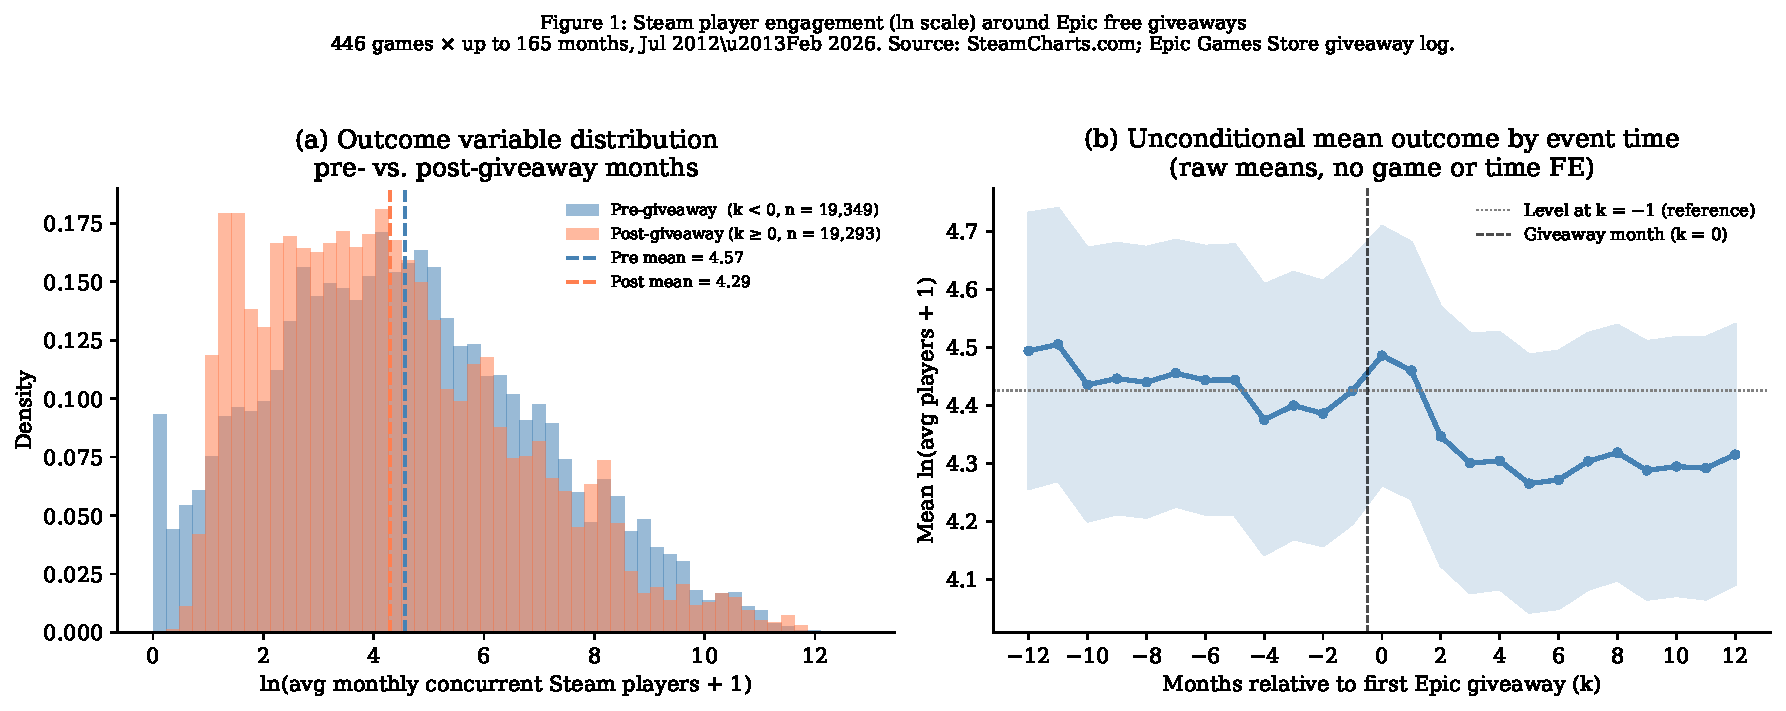
\includegraphics[width=0.88\linewidth]{../output/fig_outcome_histogram.pdf}
\caption{Steam player engagement (log scale) around Epic free giveaways.
  \textbf{Left:} Density histogram of $\ln(\avgp+1)$ for pre-giveaway
  months ($k < 0$, blue) and post-giveaway months ($k \geq 0$, orange), pooled across
  all 446 games.
  \textbf{Right:} Unconditional mean (with 95\% CI) of the outcome by event-time
  $k \in [-12,12]$; the dashed vertical line marks the giveaway month ($k = 0$).}
\label{fig:outcome}
\end{figure}

\vspace{1em}

\begin{figure}[H]
\centering
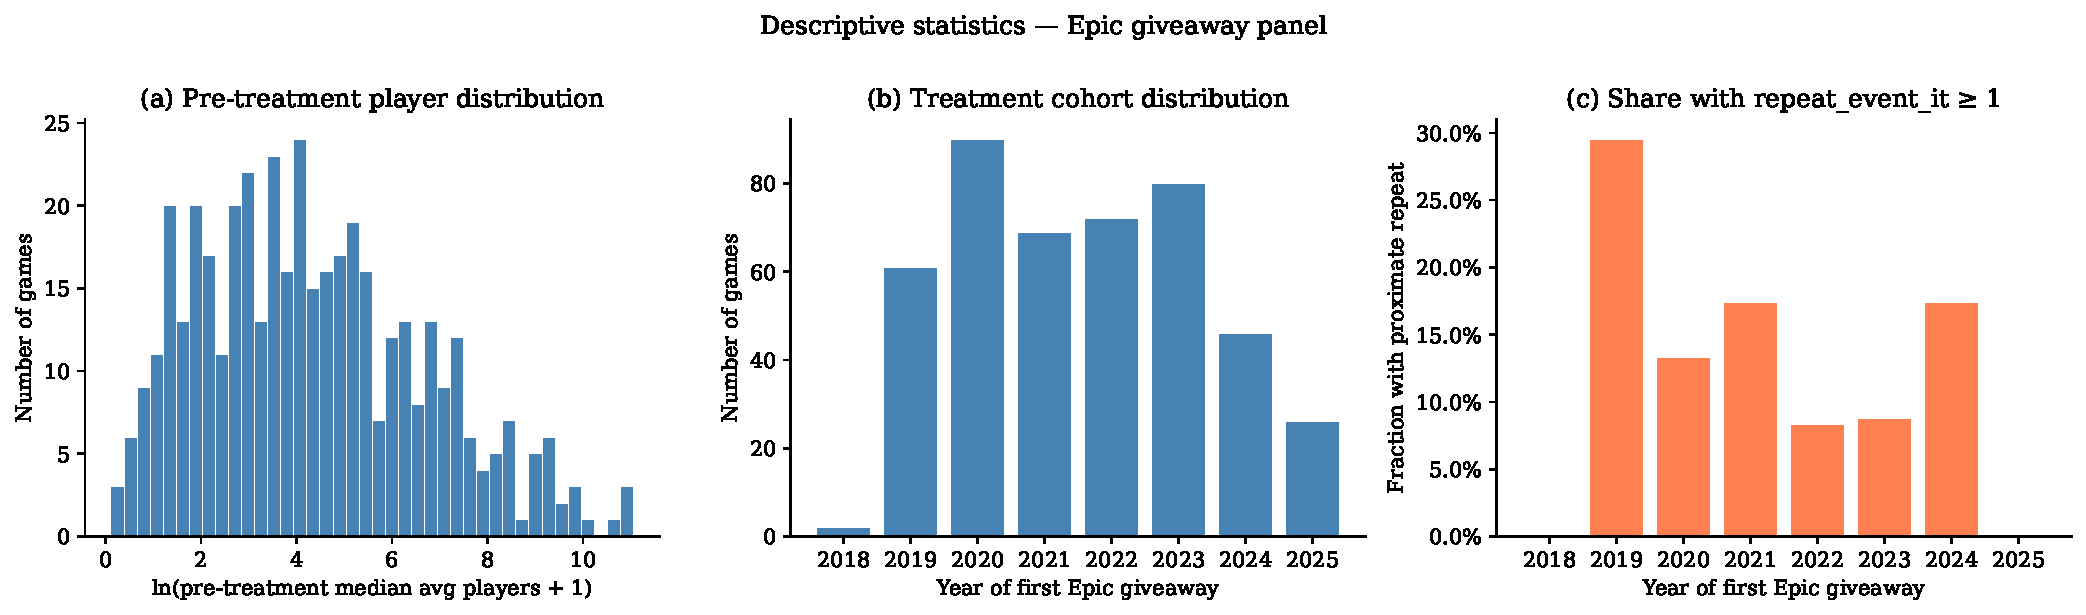
\includegraphics[width=0.88\linewidth]{../output/fig_descriptives.pdf}
\caption{Panel structure and descriptive statistics.
  \textbf{(a)} Histogram of $\ln(\text{pre-treatment median avg players} + 1)$
  across the 429 games with at least one pre-treatment observation (17 games
  whose first giveaway coincides with or precedes their earliest SteamCharts
  month have no defined pre-treatment median).
  \textbf{(b)} Number of games with first Epic giveaway in each calendar year
  (all 446 games).
  \textbf{(c)} Fraction of games in each cohort year that received a second or
  later Epic giveaway during the panel (63 games total; see
  Table~\ref{tab:epic_csv}).}
\label{fig:desc}
\end{figure}

\vspace{1em}

\begin{figure}[H]
\centering
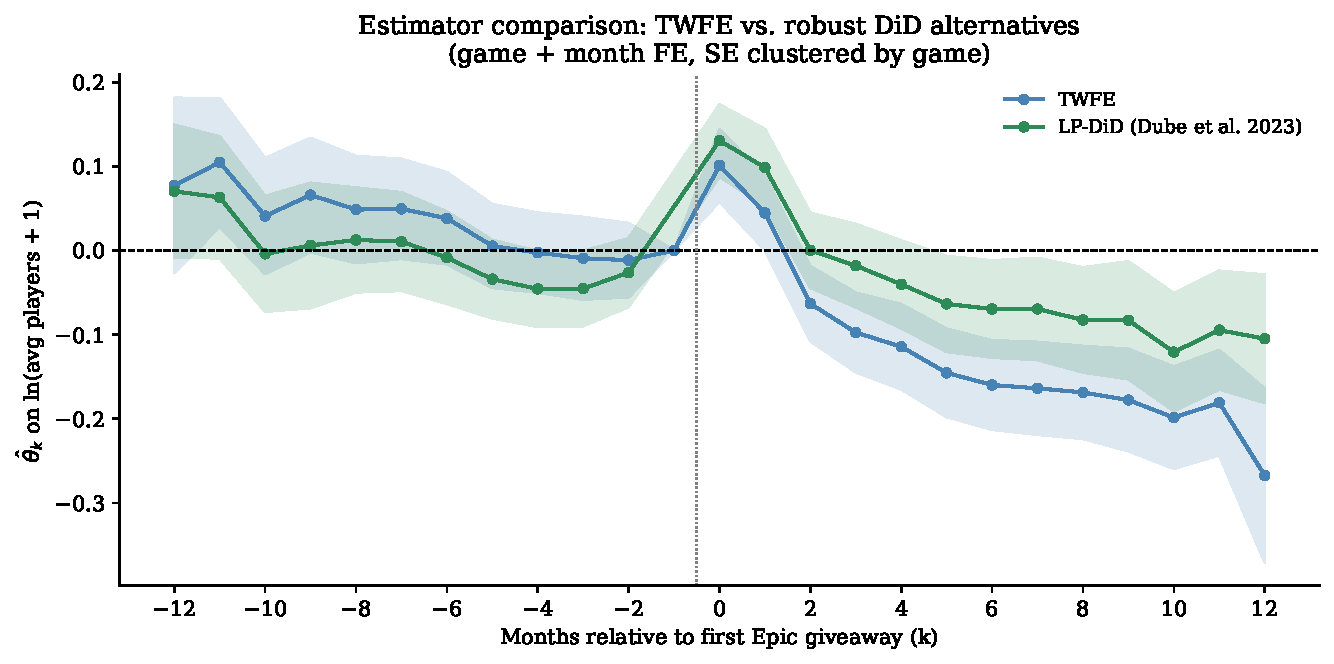
\includegraphics[width=0.82\linewidth]{../output/fig_estimator_comparison.pdf}
\caption{Event-study estimates: TWFE ($\hat{\theta}_k$, Eq.~\eqref{eq:pooled}),
  LP-DiD \citep{dube2023}, and stacked DiD \citep{cengiz2019}.
  Outcome: $\ln(\avgp+1)$.
  TWFE uses game and calendar-month fixed effects; standard errors clustered by game.
  LP-DiD uses not-yet-treated controls at each period $k$ independently.
  Stacked DiD constructs cohort-specific balanced panels with not-yet-treated
  controls, regresses $\ln(\avgp+1)$ on event-time dummies
  interacted with a treated indicator, absorbs unit-within-stack and
  stack-by-calendar-month fixed effects, and weights games appearing in
  multiple stacks by $1/n_{\text{stacks}}$.
  All estimators share the same $[-12, 12]$ event window; shaded bands are
  95\% confidence intervals. Omitted category: $k = -1$.
  $N = 38{,}641$ game-month observations; 446 games.}
\label{fig:compare}
\end{figure}

\vspace{1em}

\begin{figure}[H]
\centering
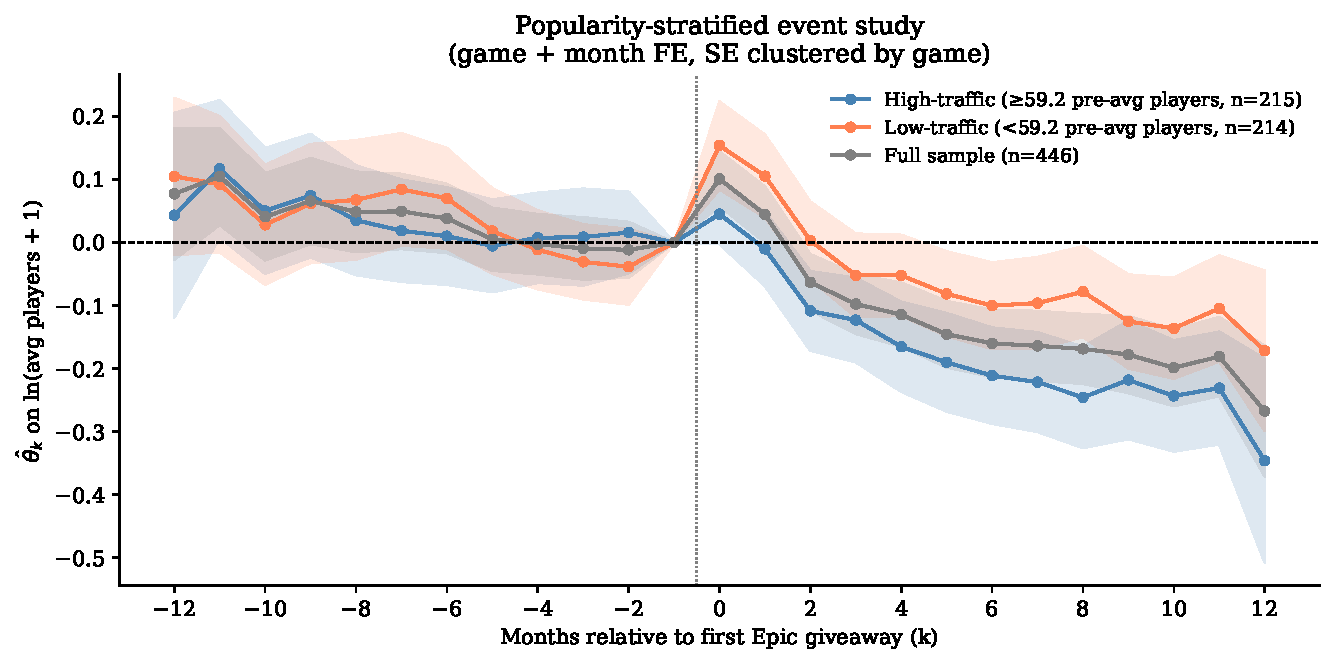
\includegraphics[width=0.88\linewidth]{../output/fig_event_study_popularity.pdf}
\caption{Event-study estimates by pre-treatment popularity. Outcome:
  $\ln(\avgp+1)$. Split at the pre-treatment median (59.2 avg
  players/month): high-traffic ($N = 215$ games) and low-traffic
  ($N = 214$ games). 17 games with no pre-period observations are
  unclassified and enter only the pooled specification. Pre-trend joint Wald
  tests: high-traffic $\chi^2_{11} = 9.04$, $p = 0.618$; low-traffic
  $\chi^2_{11} = 20.82$, $p = 0.035$.}
\label{fig:popularity}
\end{figure}

\vspace{1em}

\end{singlespace}

\clearpage

% ═══════════════════════════════════════════════════════════════════════════
%  APPENDIX
% ═══════════════════════════════════════════════════════════════════════════

\begin{singlespace}

\appendix
\renewcommand{\thesection}{\Alph{section}}
\setcounter{section}{0}

\begin{center}
{\large\bfseries Appendix}\\[0.3em]
\end{center}

\vspace{1em}

\section{Callaway--Sant'Anna Cohort ATTs}
\label{app:csatt}

We estimate cohort-specific average treatment effects $\text{ATT}(g, k)$ for each
treatment cohort $g$ (quarter of first giveaway) and event-time $k$, using
not-yet-treated games as within-cohort controls and aggregating across cohorts
weighted by cohort size \citep{callaway2021}. By conditioning on narrow
within-cohort comparisons, this estimator provides the strongest protection
against negative-weighting bias of any specification we run, at the cost of
substantially reduced precision.

Figure~\ref{fig:csatt} presents the cohort-aggregated ATT estimates. The CS
estimate at $k = 0$ is $0.048$ (SE $= 0.040$, CI $[-0.030, 0.126]$), positive in
direction but not statistically significant at conventional levels, an expected
power loss given the within-cohort design. The post-period CS estimates turn
negative from $k = 3$ onward, reaching $-0.150$ at $k = 3$ (SE $= 0.056$,
$p < 0.01$), $-0.143$ at $k = 6$, and $-0.114$ at $k = 9$. Despite the reduced
precision at $k = 0$, all four estimators (TWFE, LP-DiD, stacked DiD, and CS)
agree on the qualitative two-phase pattern.

\begin{figure}[H]
\centering
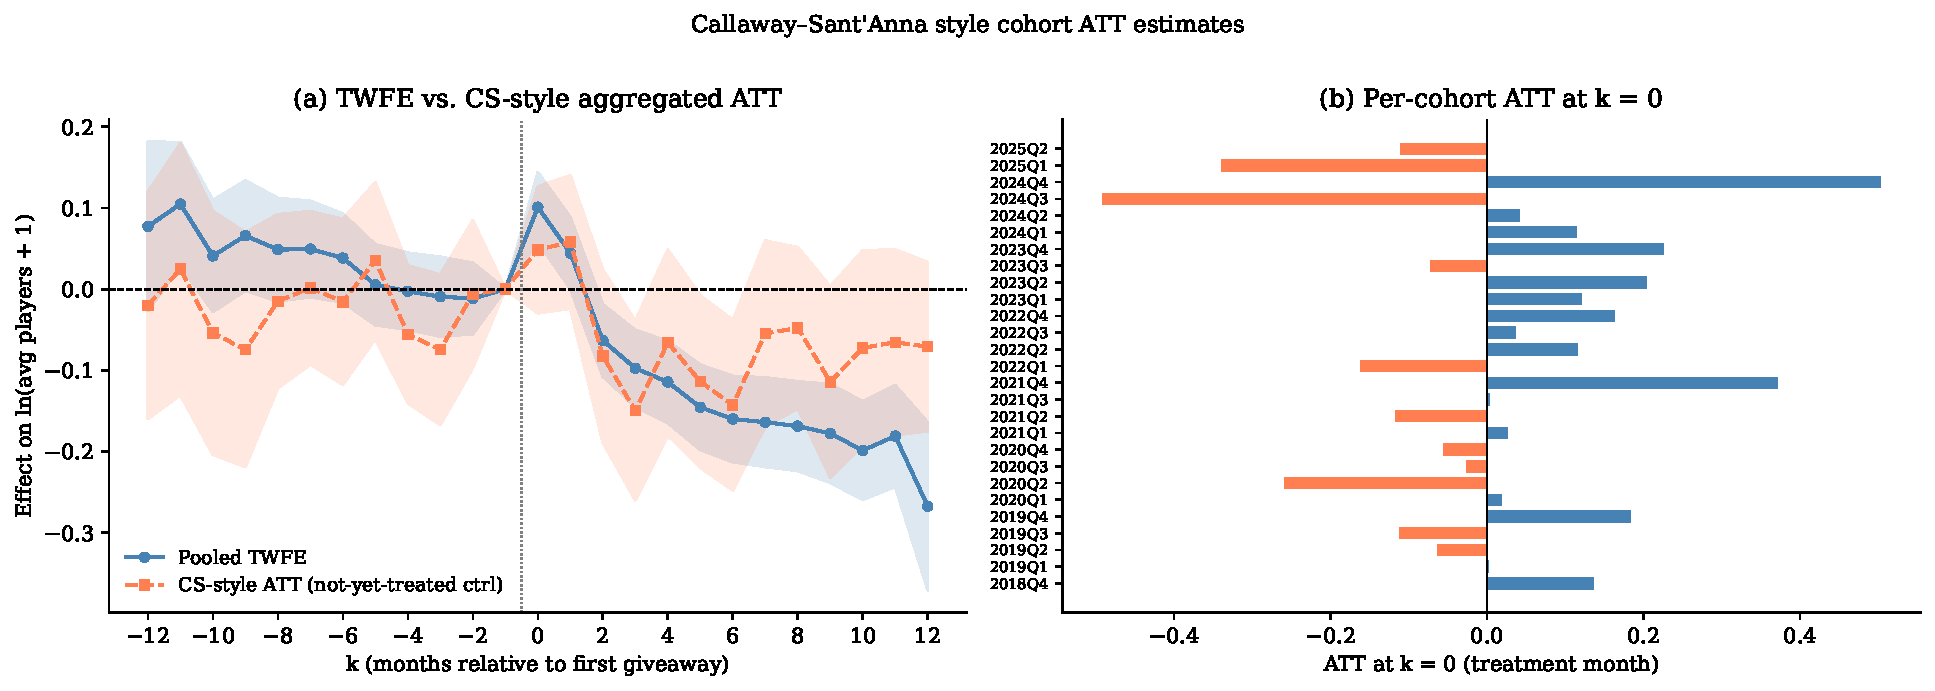
\includegraphics[width=0.82\linewidth]{../output/fig_cs_att.pdf}
\caption{Callaway--Sant'Anna cohort-aggregated ATT estimates. Outcome:
  $\ln(\avgp+1)$. Not-yet-treated games serve as controls within
  each treatment-quarter cohort; estimates are aggregated across cohorts
  weighted by cohort size. Omitted period: $k = -1$.}
\label{fig:csatt}
\end{figure}

\section{Per-Cohort Event-Study Paths}
\label{app:cohort_paths}

Figure~\ref{fig:cohort_paths} overlays the full event-study path
$\widehat{\text{ATT}}(g,k)$ for each treatment cohort, coloured from early
(dark purple) to late (bright yellow) by quarter of first-giveaway exposure.
Lines are semi-transparent to reveal the density of trajectories; the thick
black dashed line reproduces the weighted CS aggregate from
Figure~\ref{fig:csatt}. Individual cohort trajectories are highly dispersed and
noisy: some spike sharply upward at $k=0$, some show no visible jump, and a
few drift in the opposite direction. This chaos is expected: each cohort
averages only a handful of games with idiosyncratic lifecycle dynamics, so
per-cohort ATTs carry wide sampling error relative to the full-sample estimate.
The spike-and-decline pattern therefore emerges from averaging across cohorts
rather than from any individual cohort cleanly tracing it; the per-cohort
decomposition is presented here primarily to document this cohort heterogeneity.

\begin{figure}[H]
\centering
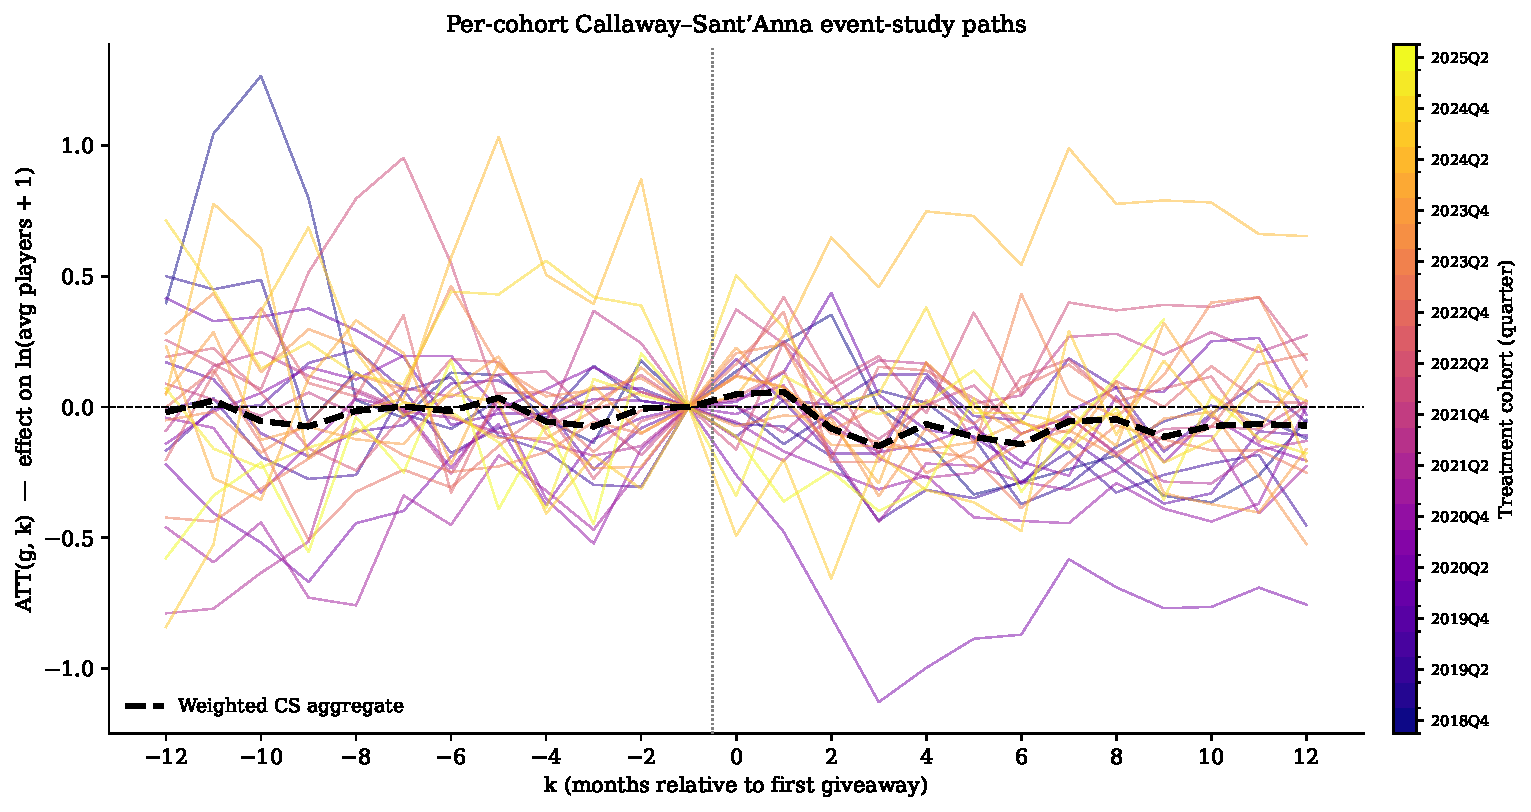
\includegraphics[width=0.88\linewidth]{../output/fig_cs_cohort_event_study.pdf}
\caption{Per-cohort Callaway--Sant'Anna event-study paths. Each thin line
  traces $\widehat{\text{ATT}}(g,k)$ for one treatment cohort $g$ across
  event times $k \in [-12,\,12]$; cohorts are coloured chronologically
  (early $\to$ late: purple $\to$ yellow).
  The thick black dashed line is the cohort-size-weighted CS aggregate.
  Vertical dotted line at $k=-0.5$ marks the pre/post boundary; horizontal
  dashed line marks zero.}
\label{fig:cohort_paths}
\end{figure}

\section{Separated Specification: First vs.\ Repeat Giveaways}
\label{app:separated}

\textbf{Specification.} To separate first-giveaway from repeat-giveaway
effects, we add a scalar indicator $\text{repeat\_event}_{it}$, equal to 1 in
any month $t$ within 12 months after game $i$'s \textit{second or later}
giveaway:
\begin{equation}
\label{eq:separated}
\ln(y_{it} + 1) = \alpha_i + \gamma_t +
  \sum_{\substack{k \in [-12,\,12] \\ k \neq -1}}
  \beta_k \cdot \mathbf{1}[\tilde{k}_{it} = k]
  \;+\;
  \delta \cdot \text{repeat\_event}_{it}
  + \varepsilon_{it}
\end{equation}
$\beta_k$ isolates the first-giveaway causal effect; $\delta$ captures the
average incremental level shift from a repeat event holding the first-event
trajectory fixed. For the 33 games with a distant repeat ($>$12 months after
the first), $\text{repeat\_event}_{it} \equiv 0$ in the event window, so
$\delta$ is identified primarily by the 30 games with a proximate
repeat.\footnote{For micro-batch repeats with gaps under one month, e.g.\
\textit{Escape Academy} re-offered within days during the 2023--2024 holiday
batch, the cluster is collapsed to its earliest date and treated as a single
event. The clean-sample specification in Appendix~\ref{app:robustness} drops
all 30 proximate-repeat games as a robustness check and leaves main estimates
unchanged.}

\textbf{Results.} The separated specification yields a repeat-giveaway
coefficient of $\hat{\delta} = 0.0001$ (SE = 0.061, $p = 0.999$, 95\% CI
approximately $[-0.12, +0.12]$). The $\hat{\beta}_k$ coefficients are
numerically identical to the pooled $\hat{\theta}_k$ to three decimal places,
as Figure~\ref{fig:separated} makes visually clear, confirming that
repeat-event contamination does not materially distort the pooled
event-study path. The wide CI on $\delta$ reflects that only 63 games
contribute identifying variation.

\textbf{Interpretation.} A zero central tendency has a clean interpretation:
the marginal player who has not yet claimed or played the game after the
first free promotion is a weak responder, and the awareness value of a second
giveaway announcement for a title already widely known to have been free is
low. The confidence interval is wide enough, however, that we cannot rule out
incremental effects of $\pm 12$ log points either way. With only 63 games
with any repeat and 30 with a proximate repeat, this null is an absence of
evidence rather than evidence of absence.

\begin{figure}[H]
\centering
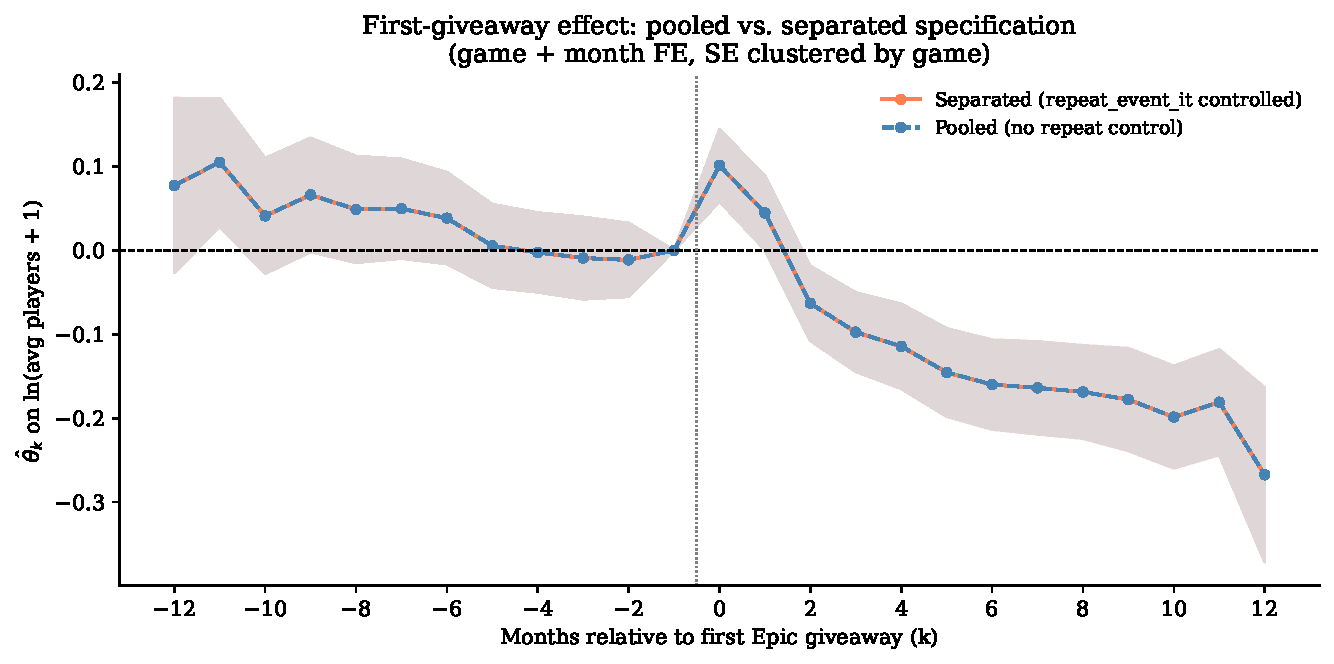
\includegraphics[width=0.82\linewidth]{../output/fig_event_study_separated.pdf}
\caption{First-giveaway event-study path under the separated and pooled
  specifications. The separated $\hat{\beta}_k$ (with the repeat-event
  indicator partialled out) and the pooled $\hat{\theta}_k$ overlay almost
  exactly, confirming that repeat-event contamination does not materially
  distort the pooled path.}
\label{fig:separated}
\end{figure}

\section{Clean-Sample Robustness Check}
\label{app:robustness}

Figure~\ref{fig:robustness} presents the pooled TWFE event-study on the clean
sample that drops all 30 games with a proximate repeat giveaway (within 12
months), leaving 416 single-event games. The coefficients are nearly identical
to the full-sample pooled TWFE (see Figure~\ref{fig:compare}), confirming that
repeat-giveaway contamination is not materially distorting the first-event
estimates.

\begin{figure}[H]
\centering
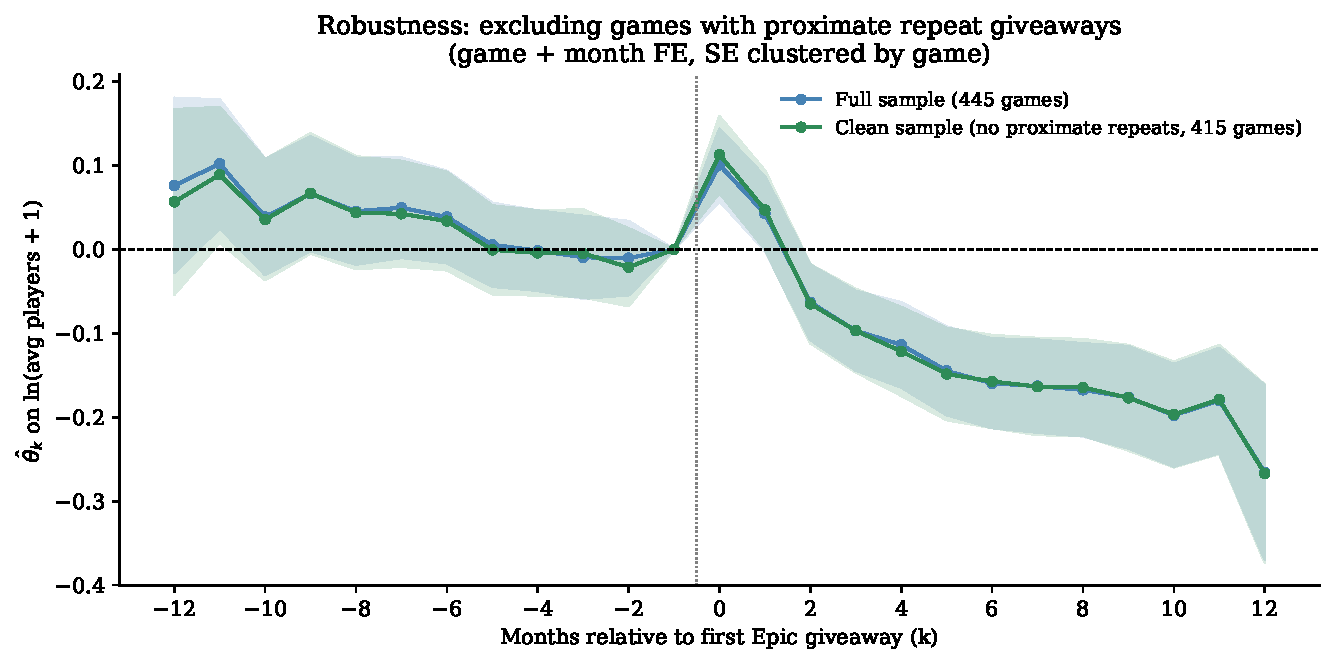
\includegraphics[width=0.82\linewidth]{../output/fig_event_study_robustness.pdf}
\caption{Clean-sample robustness check. Pooled TWFE re-estimated after dropping all 30
  games with a proximate repeat giveaway (within 12 months), leaving 416 games.
  Coefficients are virtually identical to the TWFE path in Figure~\ref{fig:compare}.}
\label{fig:robustness}
\end{figure}

\section{Holiday-Batch Robustness Check}
\label{app:holiday}

Epic's December ``15 days of free games'' batches concentrate many giveaways
into a single 2--3-week window of platform-wide media attention, so the
short-run spike could be confounded with the surrounding holiday promotional
environment. We re-estimate Equation~\eqref{eq:pooled} after dropping the 73
games whose first giveaway falls during one of these five December batches,
leaving a 373-game sample of 32{,}108 game-months. The treatment-month spike
is $+0.109$, compared with $+0.101$ in the full sample, and the $k = 12$
estimate is $-0.258$, compared with $-0.267$. Figure~\ref{fig:noholiday}
overlays the no-holiday event-study path on the full-sample TWFE estimates;
the two paths are visually indistinguishable. The advertising spike and the
medium-run decline therefore cannot be attributed to the holiday-batch media
environment: they persist at similar magnitudes when those cohorts are removed.

\begin{figure}[H]
\centering
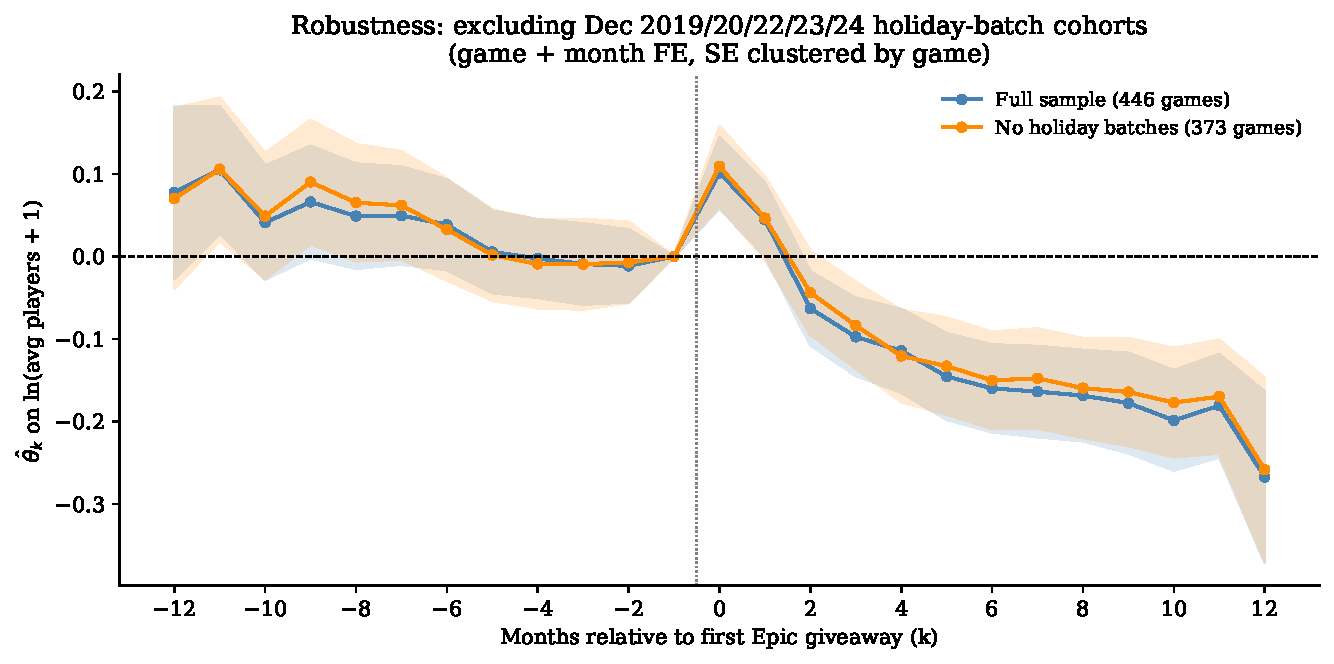
\includegraphics[width=0.82\linewidth]{../output/fig_event_study_no_holiday.pdf}
\caption{Holiday-batch robustness check. Pooled TWFE re-estimated after dropping
  the 73 games whose first giveaway falls in Epic's December holiday batches, leaving 373 games. Coefficients track the
  full-sample TWFE path closely.}
\label{fig:noholiday}
\end{figure}

\section{Randomization Placebo}
\label{app:placebo}

We permute treatment dates across all 446 games 200 times, preserving the
empirical distribution of treatment months, and re-estimate the pooled TWFE
each time. The empirical $p$-value compares the actual $|\hat{\theta}_0|$ to
the resulting permutation null. Figure~\ref{fig:placebo} shows the
distribution of $|\hat{\theta}_0|$ alongside the actual estimate: the
empirical $p$-value is $p < 0.001$, with the actual $|\hat{\theta}_0| = 0.101$
far exceeding the 95th percentile of the permutation null, 0.038. The
treatment-month spike cannot be attributed to the panel's time-series
structure or systematic calendar-time patterns alone.

\begin{figure}[H]
\centering
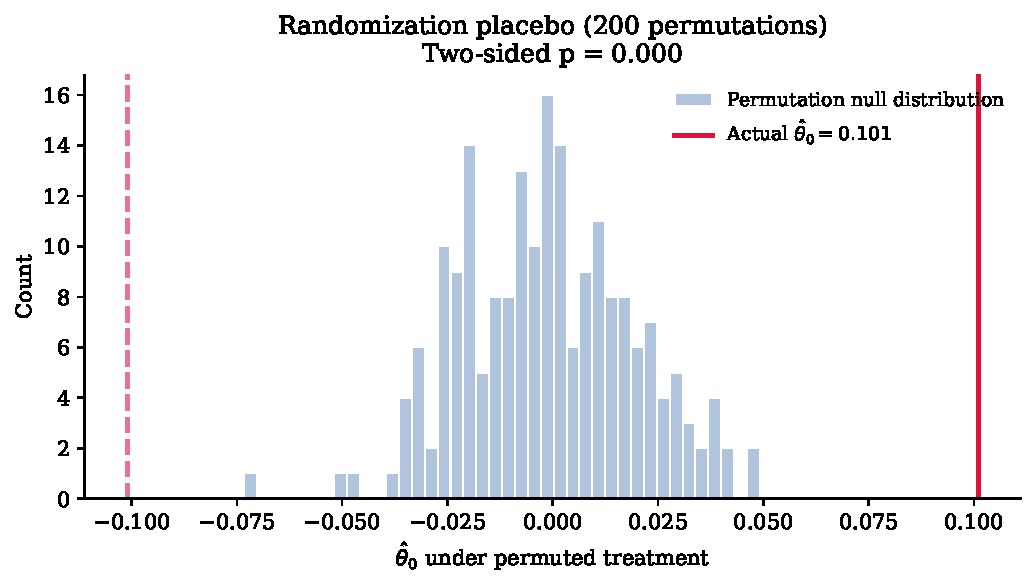
\includegraphics[width=0.72\linewidth]{../output/fig_randomization_placebo.pdf}
\caption{Randomization placebo test. Histogram of $|\hat{\theta}_0|$ from 200
  permutations of treatment dates, preserving the empirical distribution of
  treatment months. Red vertical line: actual estimate
  $|\hat{\theta}_0| = 0.101$. The 95th percentile of the permutation null is
  0.038; empirical $p < 0.001$.}
\label{fig:placebo}
\end{figure}

\section{Full TWFE Coefficient Table}
\label{app:coeftable}

Table~\ref{tab:fullcoefs} reports all 24 event-time coefficients from the pooled TWFE
specification (Equation~\eqref{eq:pooled}), including confidence intervals.

\begin{table}[H]
\centering\small
\caption{Full pooled TWFE event-study coefficients ($\hat{\theta}_k$)}
\label{tab:fullcoefs}
\begin{tabular}{rrccrr}
\toprule
$k$ & Estimate & SE & $p$-value & 2.5\% & 97.5\% \\
\midrule
$-12$ &  0.077 & 0.053 & 0.145 & $-0.027$ & 0.181 \\
$-11$ &  0.105 & 0.039 & 0.007 &    0.028 & 0.181 \\
$-10$ &  0.041 & 0.035 & 0.242 & $-0.028$ & 0.110 \\
$-9$  &  0.066 & 0.035 & 0.057 & $-0.002$ & 0.134 \\
$-8$  &  0.049 & 0.032 & 0.132 & $-0.015$ & 0.112 \\
$-7$  &  0.049 & 0.030 & 0.102 & $-0.010$ & 0.109 \\
$-6$  &  0.038 & 0.028 & 0.168 & $-0.016$ & 0.093 \\
$-5$  &  0.005 & 0.025 & 0.833 & $-0.044$ & 0.055 \\
$-4$  & $-0.003$ & 0.024 & 0.915 & $-0.050$ & 0.045 \\
$-3$  & $-0.009$ & 0.025 & 0.710 & $-0.058$ & 0.040 \\
$-2$  & $-0.011$ & 0.022 & 0.608 & $-0.055$ & 0.032 \\
$-1$  & 0 (ref) & --- & --- & --- & --- \\
\midrule
$0$  & $\mathbf{0.101}^{***}$ & 0.022 & $<$0.001 & 0.058 & 0.144 \\
$1$  & $0.045^{*}$ & 0.022 & 0.047 &  0.001 & 0.089 \\
$2$  & $-0.063^{**}$ & 0.023 & 0.005 & $-0.108$ & $-0.019$ \\
$3$  & $-0.097^{***}$ & 0.024 & $<$0.001 & $-0.145$ & $-0.050$ \\
$4$  & $-0.114^{***}$ & 0.026 & $<$0.001 & $-0.165$ & $-0.064$ \\
$5$  & $-0.145^{***}$ & 0.027 & $<$0.001 & $-0.198$ & $-0.093$ \\
$6$  & $-0.160^{***}$ & 0.027 & $<$0.001 & $-0.213$ & $-0.107$ \\
$7$  & $-0.164^{***}$ & 0.028 & $<$0.001 & $-0.219$ & $-0.109$ \\
$8$  & $-0.169^{***}$ & 0.028 & $<$0.001 & $-0.224$ & $-0.114$ \\
$9$  & $-0.178^{***}$ & 0.031 & $<$0.001 & $-0.238$ & $-0.117$ \\
$10$ & $-0.199^{***}$ & 0.031 & $<$0.001 & $-0.259$ & $-0.138$ \\
$11$ & $-0.181^{***}$ & 0.032 & $<$0.001 & $-0.243$ & $-0.119$ \\
$12$ & $-0.267^{***}$ & 0.053 & $<$0.001 & $-0.371$ & $-0.164$ \\
\bottomrule
\end{tabular}
\medskip

\noindent\small\textit{Notes:} Dependent variable: $\ln(\avgp+1)$.
  TWFE, $N = 38{,}641$; game and calendar-month fixed effects;
  standard errors clustered by game.
  $R^2 = 0.884$; within $R^2 = 0.008$.
\end{table}

\end{singlespace}

\clearpage

% ─────────────────────────── REFERENCES ────────────────────────────────────
\begin{singlespace}
\begin{thebibliography}{Callaway and Sant'Anna (2021)}
\setlength{\itemsep}{0.8em}

\bibitem[Callaway and Sant'Anna(2021)]{callaway2021}
Callaway, B.\ and Sant'Anna, P.H.C.\ (2021).
``Difference-in-Differences with Multiple Time Periods.''
\textit{Journal of Econometrics}, 225(2), 200--230.

\bibitem[Cengiz et al.(2019)]{cengiz2019}
Cengiz, D., Dube, A., Lindner, A., and Zipperer, B.\ (2019).
``The Effect of Minimum Wages on Low-Wage Jobs.''
\textit{Quarterly Journal of Economics}, 134(3), 1405--1454.

\bibitem[Clarkson(2025)]{clarkson2025}
Clarkson, T.C.\ (2025).
``Essays on Platform Operations: Applications in Service Operations and Sustainability.''
Doctoral dissertation, Moore School of Business, University of South Carolina.
Retrieved from \url{https://scholarcommons.sc.edu/etd/8313}.

\bibitem[Dongre(2025)]{dongre2025}
Dongre, P.\ (2025).
``Epic Games Free Giveaway History 2018--2025.''
Kaggle dataset. Available at
\url{https://www.kaggle.com/datasets/prajwaldongre/epic-games-free-giveaway-history-20182025}
(accessed April 2026).

\bibitem[Dub\'{e} et al.(2023)]{dube2023}
Dub\'{e}, A., Girardi, D., Jord\`{a}, O., and Taylor, A.M.\ (2023).
``A Local Projections Approach to Difference-in-Differences Event Studies.''
NBER Working Paper No.\ 31184.

\bibitem[FRVR Blog(2026)]{frvr2026}
FRVR Blog (2026).
``Epic Game Store's Free Giveaways Just Cause a Huge Spike in Steam Sales,
Reveals New Blood CEO.''
\textit{FRVR Blog}, January 20, 2026.
Retrieved from \url{https://frvr.com/blog/epic-game-stores-free-giveaways-just-causes-a-huge-spike-in-steam-sales/}.

\bibitem[Nabil and Ariatmanto(2025)]{nabil2025}
Nabil, M.\ and Ariatmanto, D.\ (2025).
``Analysis of User Satisfaction and Preferences in Choosing a Digital Game Platform
(Study Case: Steam vs Epic Games Store).''
\textit{G-Tech: Jurnal Teknologi Terapan}, 9(3), 1166--1175.

\bibitem[Reddit(2026)]{reddit2026}
Reddit (2026).
``Epic Game Store's Free Giveaways Just Cause a Huge Spike in Steam Sales.''
Posted to r/Steam, January 2026. Retrieved from
\url{https://www.reddit.com/r/Steam/comments/1qi94gk/epic_game_stores_free_giveaways_just_cause_a_huge/}.

\bibitem[Rochet and Tirole(2003)]{rochet2003}
Rochet, J.-C.\ and Tirole, J.\ (2003).
``Platform Competition in Two-Sided Markets.''
\textit{Journal of the European Economic Association}, 1(4), 990--1029.

\bibitem[Tud\'on(2022)]{tudon2022}
Tud\'on, J.\ (2022).
``Distilling Network Effects from Steam.''
\textit{Quantitative Marketing and Economics}, 20, 293--312.

\end{thebibliography}
\end{singlespace}

\vspace{1em}
\noindent\textit{Note on AI usage: I used AI to assist with drafting and formatting this
document in \LaTeX.}

\end{document}
